\documentclass{standalone}
\usepackage{amsmath}
\usepackage{amsfonts}
\usepackage{amssymb}
\usepackage{fontspec}
\usepackage{tikz}

\usetikzlibrary{arrows}
\usetikzlibrary{matrix}

\definecolor{morange}{RGB}{255,127,14}
\definecolor{mblue}{RGB}{31,119,180}
\definecolor{mred}{RGB}{214,39,40}
\definecolor{mpurple}{RGB}{148,103,189}
\definecolor{mgreen}{RGB}{44,160,44}


\begin{document}

\huge

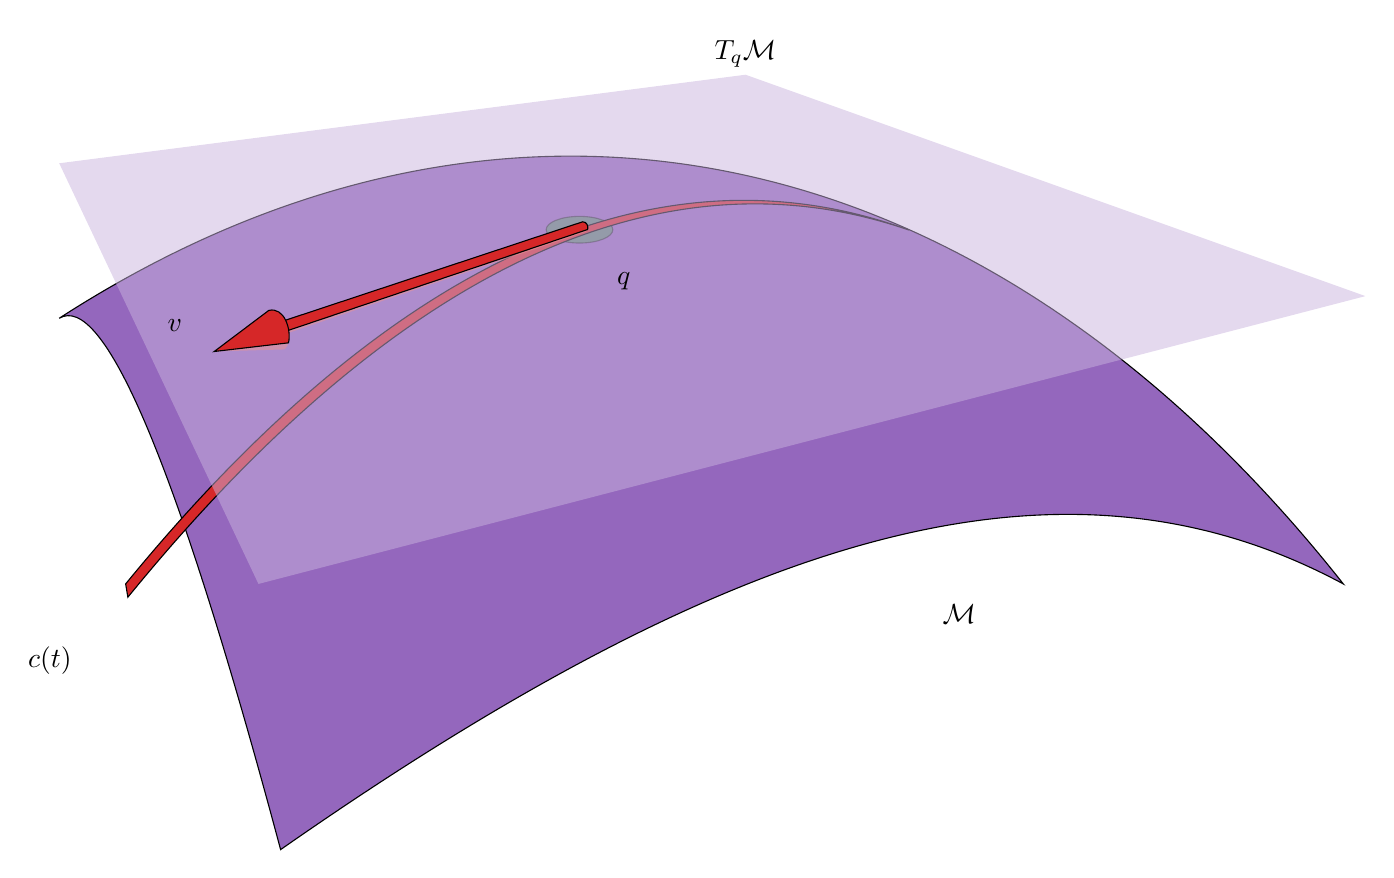
\begin{tikzpicture}[y=0.80pt, x=0.80pt, yscale=-1.000000, xscale=1.000000, inner sep=0pt, outer sep=0pt]

% manifold
\draw[fill=mpurple] (120.0000,420.0000) .. controls (71.8597,240.1403) and
  (39.4562,168.5088) .. (20.0000,180.0000) .. controls (216.5964,52.9473) and
  (434.1053,90.1579) .. (600.0000,300.0000) .. controls (472.8771,231.6315) and
  (325.8947,276.2807) .. (120.0000,420.0000) -- cycle;

% arrow base point
\draw[fill=mgreen,opacity=0.500] (255.0000,140.0000) ellipse (0.4233cm and
  0.1693cm);

% curve
\draw[fill=mred] (50.0000,300.0000) .. controls (170.0000,153.3333) and
  (290.3860,98.8070) .. (403.7193,140.1403) .. controls (291.7193,101.4737) and
  (171.6667,158.0000) .. (51.0000,306.0000) -- (50.0000,300.0000) -- cycle;

% tangent plane
\draw[fill=mpurple!50, draw opacity=0, fill opacity=0.5] (110.0000,300.0000) -- (20.0000,110.0000)
  -- (330.0000,70.0000) -- (610.0000,170.0000) -- (110.0000,300.0000);

% arrow shadow
\draw[fill=mred!50, fill opacity=0.516, draw opacity=0, line width=0.800pt, cm={{0.94667,-0.32222,0.32222,0.94667,(0.0,0.0)}}, miter limit=4.00]
  (45.3210,210.4979) -- (198.7844,211.7622) .. controls (200.5020,212.3468) and
  (201.1998,215.5767) .. (198.7844,216.4794) -- (45.6572,216.4794) --
  (45.3210,210.4979) -- cycle;

% arrow
\draw[fill=mred] (110.7360,184.6825) -- (256.4219,136.4306) .. controls (258.2362,136.4306)
  and (259.0531,138.2428) .. (258.6902,139.8983) -- (111.5302,189.5110) --
  (110.7360,184.6825) -- cycle;

% arrow tip shadow
\draw[fill=mred!50, fill opacity=0.516, draw opacity=0] (90.0000,195.0000) -- (114.6371,176.4514) .. controls (121.6667,174.6962)
  and (127.1772,189.5230) .. (121.7343,194.0800) -- (90.0000,195.0000) -- cycle;

% arrow tip
\draw[fill=mred] (90.0057,195.0148) -- (114.6429,176.4663) .. controls (121.6724,174.7110)
  and (124.9604,185.0928) .. (123.5543,191.1013) -- (90.0057,195.0148) -- cycle;


\draw[fill=black] (6.0000,341.0000)   node[above right] () {$c (t)$};
\draw[fill=black] (69.0000,186.0000)  node[above right] () {$v$};
\draw[fill=black] (272.0000,167.0000) node[above right] () {$q$};
\draw[fill=black] (316.0000,49.0000)  node[above right, yshift=-.5cm] () {${T}_{q} \mathcal{M}$};
\draw[fill=black] (419.0000,318.0000) node[above right] () {$\mathcal{M}$};

\end{tikzpicture}
\end{document}

